% Build with pdfLaTeX (twice for cross-references) or latexmk -pdf.
% The checker and its input are printed in the appendix. To regenerate those
% listings after editing the checker or grade tables, run print_verifiers.py.
\documentclass[11pt,letterpaper]{article}

% Omit the build clock and path-dependent trailer ID from the published file.
\pdfinfoomitdate=1
\pdftrailerid{}
\usepackage[
  letterpaper, left=1.02in, right=1.02in, top=0.88in, bottom=0.88in,
  headheight=14pt, headsep=15pt, footskip=28pt
]{geometry}
\usepackage[T1]{fontenc}
\usepackage{lmodern,microtype}
\usepackage{amsmath,amssymb,amsthm}
\usepackage{array,booktabs,enumitem,fancyhdr,fancyvrb,titlesec,xcolor,graphicx}

% Preserve the math extension font's delimiters and sums when text is copied.
\pdfglyphtounicode{parenleftbig}{0028}
\pdfglyphtounicode{parenrightbig}{0029}
\pdfglyphtounicode{parenleftbigg}{0028}
\pdfglyphtounicode{parenrightbigg}{0029}
\pdfglyphtounicode{summationtext}{2211}
\pdfglyphtounicode{summationdisplay}{2211}

\definecolor{ink}{HTML}{17515A}
\definecolor{grayink}{HTML}{4A5659}
\definecolor{panel}{HTML}{EDF4F3}
\definecolor{panelrule}{HTML}{B8D0CE}

\usepackage[colorlinks=true,linkcolor=ink,citecolor=ink,urlcolor=ink,bookmarksnumbered=true]{hyperref}
\newcommand{\papertitle}{Elections with Condorcet Dimension 4}
\hypersetup{
  pdftitle={\papertitle},
  pdfsubject={Coverage bounds for Condorcet committees}
}

\pagestyle{fancy}
\fancyhf{}
\fancyhead[L]{\small\color{grayink}\papertitle}
\fancyhead[R]{\small\color{grayink}\nouppercase{\rightmark}}
\fancyfoot[C]{\small\thepage}
\renewcommand{\headrulewidth}{0.3pt}
\renewcommand{\sectionmark}[1]{\markright{\thesection\enspace #1}}
\renewcommand{\subsectionmark}[1]{}

\titleformat{\section}{\large\bfseries\color{black}}{\thesection}{0.6em}{}
\titlespacing*{\section}{0pt}{14pt plus 3pt minus 2pt}{5pt plus 1pt}
\titleformat{\subsection}{\normalsize\bfseries\color{ink}}{\thesubsection}{0.55em}{}
\titlespacing*{\subsection}{0pt}{10pt plus 2pt minus 1pt}{3pt plus 1pt}

\setlength{\parindent}{0pt}
\setlength{\parskip}{4.8pt plus 0.6pt minus 0.3pt}
\setlength{\abovedisplayskip}{7pt plus 2pt minus 2pt}
\setlength{\belowdisplayskip}{7pt plus 2pt minus 2pt}
\setlength{\abovedisplayshortskip}{4pt}
\setlength{\belowdisplayshortskip}{4pt}
\raggedbottom
\widowpenalty=8000
\clubpenalty=8000

\setlist[itemize]{leftmargin=1.4em,itemsep=3pt,topsep=3pt,parsep=0pt}
\setlist[enumerate]{leftmargin=1.6em,itemsep=3pt,topsep=3pt,parsep=0pt}

\newtheoremstyle{cleanthm}{8pt}{6pt}{\itshape}{}{\bfseries}{.}{0.5em}{}
\theoremstyle{cleanthm}
\newtheorem{theorem}{Theorem}
\newtheorem{lemma}{Lemma}
\newtheorem{proposition}[lemma]{Proposition}
\newtheorem{corollary}[lemma]{Corollary}

\newcommand{\lead}[1]{\textbf{#1}\enspace}
\newcommand{\FULL}{\mathrm{FULL}}
\newcommand{\TIE}{\mathrm{TIE}}
\newcommand{\TARGET}{\mathrm{TARGET}}
\newcommand{\jointnum}{351449648252133}
\newcommand{\jointden}{512000000000000}

\begin{document}

% ============================================================================
% Introduction and main result
% ============================================================================

\thispagestyle{plain}\pdfbookmark[1]{Introduction and main result}{opening}
{\centering
  {\LARGE\papertitle\par}
  \vspace{8pt}
  {\large November 20, 2026\par}
}
\vspace{5pt}

\begin{abstract}
A committee wins if, against each outsider, a strict majority of voters prefer at least one committee member to that outsider. We construct a finite ranked election in which every three-member committee faces a single outsider preferred to all three by more than \(51.48\%\) of the voters. Thus four candidates can be necessary. More generally, for every \(k\ge2\) there are elections in which every \(k\)-member committee faces such opposition from more than a \(2.059275/(k+1)\) fraction of the voters. This disproves the conjecture of Charikar, Lassota, Ramakrishnan, Vetta, and Wang that the factor \(2\) in Zbarsky's lower bound \(2/(k+1)\) is optimal. Our construction lets a single candidate break ties against different opponents on different ballots. Two small grade tables give a hand proof of the majority obstruction. An exact certificate gives the stated numerical bound.
\end{abstract}
\begin{quote}
\small
\noindent\textbf{Note:}
This manuscript was generated by AI with minimal human input and intentionally has no human author. GPT-6.2 Astra developed the original proofs. Gemini 4 Carbon and Neon helped revise the writing. The proofs have been formalized in lean, and are available here \mbox{[Lean proof link]}.

\smallskip\noindent
In the spirit of \href{https://theorydish.blog/2026/11/18/a-friendlier-equilibrium-for-sharing-research/}{this blog post}, the contributors are organizing a collaboration to extend these results and produce a high-quality, human-written exposition. We invite interested researchers to \href{https://condorcetsets.zulipchat.com/join/vokzarv7flx54z7hkk3gjaij/}{join us on Zulip}. If the invitation has expired, please email \mbox{\href{mailto:pras_r@seas.harvard.edu}{\nolinkurl{pras_r@seas.harvard.edu}}}.
\end{quote}

\section*{Introduction}
Each of finitely many voters strictly ranks the same finite set of candidates. A committee \(S\)
\emph{covers} a voter against an outsider \(h\) if the voter ranks some member of \(S\) above
\(h\). A \emph{Condorcet winning set} covers a strict majority against each outsider~\cite{els}.
A result of Jiang, Munagala, and Wang~\cite{jmw} on approximately stable committees implies
that every election has a Condorcet winning set of at most 32 candidates.
Charikar, Lassota, Ramakrishnan, Vetta, and Wang~\cite[Section~1.1]{clrv} observed this
implication and proved that six candidates suffice.
Song, Nguyen, and Lin~\cite{snl} reduced this to five. Prasanna Ramakrishnan~\cite{ram} gives a
short proof using Brouwer's fixed-point theorem.

Write \(p_E(h,S)\) for the fraction of voters in election \(E\) who rank \(h\) above every member
of \(S\). The \emph{opposition} to \(S\) is \(\max_{h\notin S}p_E(h,S)\). For \(k\ge1\), define
\[
 A_k=\sup_E\,\min_{|S|=k}\,\max_{h\notin S}p_E(h,S),
 \qquad C_k=\inf_E\,\max_{|S|=k}\,\min_{h\notin S}\bigl(1-p_E(h,S)\bigr)=1-A_k,
\]
where \(E\) ranges over elections with at least one voter and more than \(k\) candidates. In each
such election some \(k\)-member committee covers at least a fraction \(C_k\) of voters against
each outsider. This is the largest universal guarantee. Enlarging a committee weakly decreases its
opposition, so committees of size at most \(k\) give the same values. Nonnegative rational ballot
weights summing to~\(1\) describe a finite electorate after clearing denominators.

Sam Zbarsky's cyclic construction~\cite{zbarsky} gives \(A_k\ge 2/(k+1)\) for general \(k\)
(see~\cite[Theorem~7]{clrv}). Jiang, Munagala, and Wang~\cite{jmw} use a related construction for
committee stability. Conjecture~1 of~\cite{clrv} asks whether every election admits a \(k\)-member
committee with opposition below \(2/(k+1)\).

\begin{center}
\setlength{\fboxsep}{9pt}
\fcolorbox{panelrule}{panel}{\begin{minipage}{.92\linewidth}
\begin{theorem}\label{thm:main}
For every integer \(k\ge 2\),
\[
 C_k \;\le\; 1-\frac{3A_2}{k+1} \;\le\; 1-\frac{3z}{k+1},
 \qquad z=\frac{\jointnum}{\jointden}=0.686425094242\ldots\,.
\]
In particular, \(C_2<1/3\), \(C_3<1/2\), and \(\liminf_{k\to\infty} k(1-C_k)\ge 3z > 2.059275\).
\end{theorem}
\end{minipage}}
\end{center}

For each \(k\ge2\) and \(\varepsilon>0\), there is a finite election in which every \(k\)-member
committee faces opposition at least \(3z/(k+1)-\varepsilon\). Taking
\(0<\varepsilon<(3z-2)/(k+1)\) disproves the conjecture for every \(k\ge2\). In particular,
\(3z/4>0.5148\), so there is a single finite election in which every triple faces an outsider whom
more than \(51.48\%\) of voters rank above all three members. The outsider may depend on the
triple. The \emph{Condorcet dimension} is the size of an election's smallest winning set. Its
largest possible value is therefore four or five.

\begin{center}
\setlength{\tabcolsep}{9pt}\renewcommand{\arraystretch}{1.13}
\begin{tabular}{@{}c c c r@{}}
\toprule
& \multicolumn{3}{c}{Upper bounds on the universal coverage guarantee \(C_k\)}\\
\cmidrule(l){2-4}
Seats \(k\) & Cyclic bound \(1-2/(k+1)\) & Theorem~\ref{thm:main} & Rounded up\\
\midrule
2 & \(1/3\) & \(1-z\)      & \(31.36\%\)\\
3 & \(1/2\) & \(1-3z/4\)   & \(48.52\%\)\\
4 & \(3/5\) & \(1-3z/5\)   & \(58.82\%\)\\
5 & \(2/3\) & \(1-z/2\)    & \(65.68\%\)\\
\bottomrule
\end{tabular}
\end{center}

\begin{figure}[htbp]
\centering
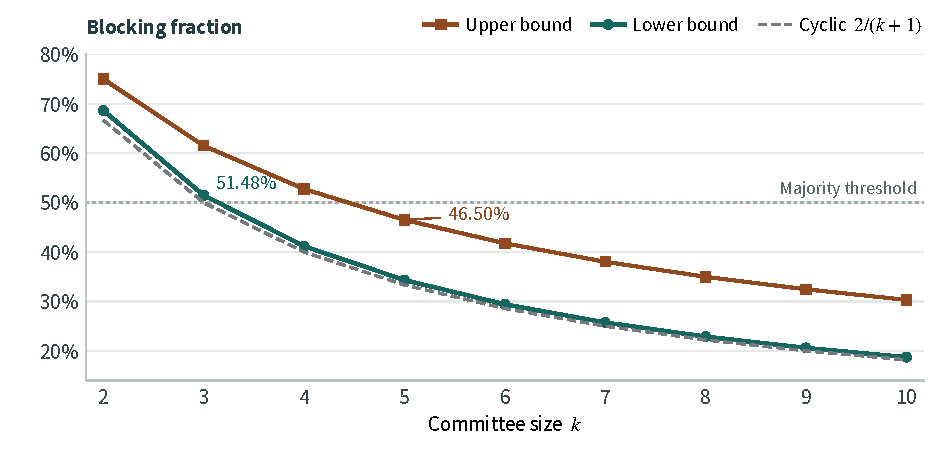
\includegraphics[width=.91\linewidth]{small-committee-bounds.pdf}
\caption{Bounds on opposition \(A_k=1-C_k\) for committees of two to ten candidates. The lower bound is \(3z/(k+1)\) from Theorem~\ref{thm:main}. The upper bound is \(1-(1-1/k)k^{-1/(k-1)}\) from Song, Nguyen, and Lin~\cite{snl}. The dashed gray curve is Zbarsky's cyclic bound~\cite{zbarsky}.}
\label{fig:small-bounds}
\end{figure}

% ============================================================================
% Section 1: From grade tables to strict elections
% ============================================================================

\clearpage
\section[Grade tables to strict elections]{From grade tables to strict elections}\label{sec:refinement}

A challenger can tie different rivals for the best grade at different voter positions. To break
these ties, we use a strict \emph{inner election} and let each candidate choose a name from that
election separately at each position. We first bound the support available against several rivals
at one position.

\begin{lemma}[Repeated inner challenges]\label{lem:transitive}
Let \(E\) be a finite strict election with at least three candidates and \emph{pair opposition at
least \(a\)}: every pair has an outsider who beats it on at least a fraction \(a\in[0,1]\) of the
ballots. Given any list \(u_1,\ldots,u_i\) of \(i\ge2\) candidates, with repetitions allowed, some
candidate beats them all on a fraction of ballots at least
\[
     c_i(a)=\max\{0,\,1-(i-1)(1-a)\}.
\]
\end{lemma}

\begin{proof}
For \(i=2\), two distinct candidates form a pair. If \(u_1=u_2\), pair \(u_1\) with any other
candidate of \(E\) and use that pair's challenger. In either case the success fraction is at least
\(a\).

For the induction step, suppose \(1-(i-1)(1-a)>0\), since a lower bound of zero is automatic. By
induction some candidate \(w\) beats \(u_1,\ldots,u_{i-1}\) on at least \(1-(i-2)(1-a)\) of the
ballots. Apply the \(i=2\) case to \(w\) and \(u_i\). On the ballots where both challenges
succeed, transitivity puts the second challenger above all \(i\) candidates. The two sets of
supporting ballots overlap on a fraction at least
\[
 1-(i-2)(1-a)+a-1 = 1-(i-1)(1-a). \qedhere
\]
\end{proof}

Set \(c_0(a)=c_1(a)=1\), and abbreviate \(c_i(a)\) to \(c_i\) when \(a\) is fixed. For \(a\ge 2/3\),
\begin{equation}\label{eq:tie-credits}
 (c_0,c_1,c_2,c_3,c_4)=(1,1,a,2a-1,3a-2).
\end{equation}

\lead{Grade tables.}
A \emph{grade table} consists of a finite nonempty list of voter positions with nonnegative
rational weights summing to~\(1\), together with a finite nonempty set of allowed \emph{grade
assignments}. Each grade assignment gives a grade (from a fixed ordered list, with \emph{smaller}
grades preferred) to every position. In the small constructions, each type has one assignment. In
the certificate, each type has a menu of permitted choices for each row. A complete assignment
specifies the option for each row and the set of marked positions wherever the option leaves that
set free.

Fix \(a\in[0,1]\), a list of \(k\ge1\) rival assignments (repeats allowed), and a challenger
assignment. At each position give the challenger credit \(1\) if it beats every rival in grade,
\(0\) if a rival has a better grade, and \(c_i(a)\) if exactly \(i\) rivals tie it for best grade.
Its \emph{table score} is the weighted sum of these credits.

\begin{lemma}[Turning a grade table into a strict election]\label{lem:refine}
Fix a grade table, an integer \(k\ge 1\), and a finite strict election \(E\) with at least three
candidates and pair opposition at least \(a\in[0,1]\). Let \(M\) be the minimum over all
\(k\)-tuples of rival grade assignments (repeats allowed) of the maximum table score over all
challenger grade assignments. For every integer \(L\ge 2\) with \(3L>k\), there is a finite strict
election with more than \(k\) candidates in which every \(k\)-member committee faces opposition at
least \(M-1/L\). Letting \(L\to\infty\) gives
\begin{equation}\label{eq:refine-limit}
 A_k \;\ge\; M.
\end{equation}
\end{lemma}

\begin{proof}
Replace each candidate \(u\) of \(E\) by \(L\) clones \((u,r)\) with \(r\in\{0,\ldots,L-1\}\). A
candidate in the new election chooses one allowed grade assignment and, independently at each
position, one inner clone \((u,r)\). Include every such combination. Because there is at least one
position, at least one allowed grade assignment, and at least \(3\) candidates in \(E\), the new
election is finite and has at least \(3L>k\) candidates.

Independently draw a position according to its weight, a uniformly chosen voter of \(E\), and a
uniform shift \(s\in\{0,\ldots,L-1\}\). At the drawn position rank the candidates by increasing
grade, then by the inner voter's ranking of \(u\), then by increasing \((r+s)\bmod L\). A fixed
strict order breaks any remaining ties. All draws have rational probabilities, so these ballots
form a finite strict election.

Fix a \(k\)-member committee \(S\) and choose a challenger grade assignment whose table score
against the grade assignments of \(S\) is at least \(M\). Choose its inner clone at each position
as follows.
\begin{itemize}
 \item With a strictly better grade than all rivals, any clone wins. With a strictly worse grade
   than the best rival, any clone gives the claimed lower bound of zero.
 \item With one tied rival, whose clone here is \((u,r)\), take its predecessor
   \((u,(r-1)\bmod L)\). This clone beats it except on the one shift for which \((r+s)\bmod L=0\),
   and beats the other rivals by grade. Its success fraction is \(1-1/L\).
 \item With \(i\ge2\) rivals tied for best grade, apply Lemma~\ref{lem:transitive} to their inner
   candidates, allowing repetitions. Any clone of the resulting candidate of \(E\) beats all tied
   rivals on at least a fraction \(c_i(a)\) of the ballots here and beats every worse-graded rival
   on all of them.
\end{itemize}
Because every combination of clones is included, these choices define one candidate. Only
positions with a single tied rival can fall short of their table credit, by \(1/L\) each. Their
total weight is at most~\(1\), so the candidate beats \(S\) on at least a fraction \(M-1/L\) of
all ballots. If \(M-1/L>0\), at least one ballot ranks it strictly above every member of \(S\), so
it is an outsider. If \(M-1/L\le0\), any outsider suffices and one exists because the election has
more than \(k\) candidates.
\end{proof}

For two rivals and one challenger in a fixed table, write \(w\) for the weight of positions where
the challenger beats both rivals or ties one and beats the other, \(t\) for the weight where all
three grades tie, and \(d=1-w-t\) for the weight where a rival has a better grade. Define \(F(x)\)
for \(x\in[0,1]\) as the minimum over all pairs of rival grade assignments (repeats allowed) of
the maximum of \(w+tx\) over all challenger grade assignments.

\begin{corollary}[Self-improvement for pairs]\label{cor:self}
For every grade table,
\begin{equation}\label{eq:self}
 A_2 \;\ge\; F(A_2).
\end{equation}
Fix \(\theta\in(0,1]\).
\begin{enumerate}[label=\textup{(\alph*)}]
 \item If every rival pair has a challenger with \(w+d>0\) and \(w\ge \theta(w+d)\), then
   \(A_2\ge \theta\).
 \item If every rival pair has a challenger with \(w>\theta(w+d)\), then \(A_2>\theta\).
\end{enumerate}
\end{corollary}

\begin{proof}
Take a sequence of finite elections with at least three candidates whose minimum pair oppositions
\(a_n\) tend to \(A_2\), as permitted by the definition of the supremum.
Applying~\eqref{eq:refine-limit} with \(k=2\) to each election gives \(A_2\ge F(a_n)\). A finite
minimum of finite maxima of affine functions is continuous. Passing to the limit
gives~\eqref{eq:self}.

Since \(t=1-w-d\), the gain in score over \(x\) is \(w+tx-x=w-(w+d)x\). Under~(a), this gain is at
least \((w+d)(\theta-x)>0\) for all \(x\in[0,\theta)\). Under~(b), since \(w+d\ge 0\), it is at
least \(w-(w+d)\theta>0\) for all \(x\in[0,\theta]\). Since there are only finitely many rival
pairs, \(F(x)>x\) throughout each range, and~\eqref{eq:self} excludes \(A_2\) from it.
\end{proof}

% ============================================================================
% Section 2: Short proofs by hand
% ============================================================================

\newpage
\section[Short proofs by hand]{Short proofs by hand that \texorpdfstring{\(C_2<1/3\)}{C2 < 1/3} and \texorpdfstring{\(C_3<1/2\)}{C3 < 1/2}}\label{sec:thresholds}

Before proving the numerical bound in Theorem~\ref{thm:main}, we give two small constructions that
can be checked by hand and already beat the cyclic bounds \(1/3\) for pairs and \(1/2\) for
triples.

\begin{proposition}\label{prop:pair-third}
We have \(A_2>2/3\), and so \(C_2<1/3\).
\end{proposition}

\begin{proof}
Take twelve candidate types numbered \(0,1,\ldots,11\) modulo~\(12\), each with one grade
assignment. Use the three length-12 grade words below (smaller digit preferred) with the listed
relative weights:
\[
\begin{array}{l@{\quad}c@{\quad}r}
 \text{Word} & \text{Digits in positions } 0,1,\ldots,11 & \text{Weight}\\\midrule
 \text{Word 1} & \mathtt{501401301201} & 64\\
 \text{Word 2} & \mathtt{201000200001} & 16\\
 \text{Word 3} & \mathtt{501234501234} & 1
\end{array}
\]
Each word produces twelve voter positions indexed by shifts \(s=0,1,\ldots,11\): on shift \(s\),
type \(j\) gets the digit at index \((j+s)\bmod 12\), and each shift has the listed relative
weight. Dividing by the total weight \(12(64+16+1)=972\) makes the \(36\) position weights sum
to~\(1\).

Adding the same offset modulo~\(12\) to the rivals and challenger only permutes the twelve shifts
of each word, so we may translate either rival to type~0. Choosing which rival to translate
represents every pair as \(\{0,r\}\) for some \(0\le r\le 6\) (including \(r=0\) for two rivals of
the same type). For a challenger type \(h\) and one word, call a shift \(s\) a \emph{win} if the
digit at \((s+h)\bmod 12\) is at most the smaller of the digits at \(s\) and \((s+r)\bmod 12\),
without all three being equal, and a \emph{loss} if it is strictly larger than that minimum. The
table lists \((\text{wins})-2(\text{losses})\) for each word and their weighted sum (\(64\) times
Word~1, plus \(16\) times Word~2, plus Word~3):

\begin{center}\small
\setlength{\tabcolsep}{10pt}\renewcommand{\arraystretch}{1.12}
\begin{tabular}{@{}c c rrr r@{}}
\toprule
Distance \(r\) & Challenger \(h\) & Word 1 & Word 2 & Word 3 & Weighted sum\\
\midrule
0 & 3  & 1 & \(-3\) & \(-6\)  & 10\\
1 & 3  & 0 & \(1\)  & \(-12\) & 4\\
2 & 11 & 0 & \(1\)  & \(-6\)  & 10\\
3 & 3  & 1 & \(-3\) & \(-6\)  & 10\\
4 & 9  & 0 & \(1\)  & \(-6\)  & 10\\
5 & 8  & 0 & \(1\)  & \(-12\) & 4\\
6 & 5  & 0 & \(0\)  & \(6\)   & 6\\
\bottomrule
\end{tabular}
\end{center}

For example, at \(r=0\) and \(h=3\), the digits in Word~1 differ only on \(s\in\{0,3,6,9\}\).
There the challenger beats the rivals on \(s=0,3,6\) (\(4<5\), \(3<4\), \(2<3\)) and loses on
\(s=9\) (\(5>2\)), giving \(3-2(1)=1\). Every other entry is checked in the same way by comparing
the digits at \((s+h)\bmod 12\), \(s\), and \((s+r)\bmod 12\) for \(s=0,\ldots,11\).

Let \(W\) and \(D\) be the weighted totals of wins and losses across all \(36\) positions, so
\(w=W/972\) and \(d=D/972\). Because \(W-2D\ge 4>0\) in every row of the table,
\[
 w - \frac{2}{3}(w+d) \;=\; \frac{W-2D}{3\cdot 972} \;\ge\; \frac{4}{3\cdot 972} \;=\;
 \frac{1}{729} \;>\; 0
\]
for every rival pair. Corollary~\ref{cor:self}(b) with \(\theta=2/3\) gives \(A_2>2/3\), so
\(C_2<1/3\).
\end{proof}

\newpage
\lead{Earlier pair constructions.}
Elkind, Lang, and Saffidine~\cite[Proposition~6]{els11} gave a 15-candidate election, built from
three cyclic blocks of five candidates, where every pair is beaten by one outsider on at least 8
of 15 ballots. More generally, use three cyclic blocks of \(N\ge2\) candidates. The \(3N\) ballots
use every outer and inner rotation, with the same inner rotation in each block. If both rivals are
in one block, any candidate in the preceding block beats them on \(2N\) ballots. If the rivals lie
in different blocks, one rival's block precedes the other's in two outer rotations; in both, the
cyclic predecessor of that first rival beats the other rival by block and beats the first rival in
\(N-1\) inner rotations, giving \(2(N-1)\) wins out of \(3N\) ballots. Letting \(N\) grow gives
\(A_2\ge 2/3\).

Elkind, Lang, and Saffidine~\cite[pp.~500, 516]{els} report two further strict-majority examples
from personal communications. Cervone and Zwicker found one with 11 candidates and 11 voters in
2011. Cervone, Hardin, and Zwicker found one with 7 candidates and 21 voters in 2012 (see
also~\cite{chz}). David E.~Speyer~\cite{speyer} posted a 7-candidate example in 2013 in which
every pair is beaten on 11 of 21 ballots. In Christian Geist's 6-candidate, 6-voter
example~\cite[Fig.~2]{geist}, every pair faces opposition of exactly one half, enough to prevent a
strict majority for the pair.

\begin{proposition}\label{prop:triple-half}
We have \(A_3\ge (1+3A_2)/6 > 1/2\), and so \(C_3<1/2\).
\end{proposition}

\begin{proof}
By Proposition~\ref{prop:pair-third}, we can fix \(2/3<a<A_2\) and take an inner election with
pair opposition at least \(a\). By~\eqref{eq:tie-credits}, \(c_0=c_1=1\), \(c_2=a\), and
\(c_3=2a-1\).

Split six candidate types into two groups \(X=\{x_0,x_1,x_2\}\) and \(Y=\{y_0,y_1,y_2\}\) of three
types each. Use six equally weighted positions (weight \(1/6\) each):
\begin{itemize}
 \item Three \emph{\(X\)-rows}, giving grades \((0,1,2)\), \((2,0,1)\), and \((1,2,0)\) to
   \((x_0,x_1,x_2)\) and grade~\(0\) to all of \(Y\).
 \item Three \emph{\(Y\)-rows}, swapping the roles of \(X\) and \(Y\).
\end{itemize}
Given any three rival types (repeats allowed), by symmetry we may assume that at least two lie in
\(X\). We sum the credits over all six rows before dividing by~\(6\):
\begin{itemize}
 \item \emph{Two rivals in \(X\) and one in \(Y\).} Challenge with a type in \(Y\) different from
   the \(Y\)-rival. On the three \(X\)-rows, the challenger has grade~\(0\) and ties the
   \(Y\)-rival plus whichever \(X\)-rivals have grade~\(0\); the tie counts on the three rows are
   either \(3,1,1\) (credit \((2a-1)+1+1=1+2a\)) or \(2,2,1\) (credit \(a+a+1=1+2a\)). On the
   \(Y\)-row where the challenger has grade~\(0\), the \(Y\)-rival has grade \(1\) or \(2\) while
   both \(X\)-rivals have grade~\(0\), adding \(c_2=a\). The total is \(1+3a\).
 \item \emph{Three rivals in \(X\), of at least two types.} Challenge with any type in \(Y\). On
   the three \(X\)-rows, the challenger has grade~\(0\) and ties whichever rivals have
   grade~\(0\); the tie counts on the three rows are either \(2,1,0\) (credit \(a+1+1=2+a\)) or
   \(1,1,1\) (credit \(3>2+a\)). On the \(Y\)-row where the challenger has grade~\(0\), it ties
   all three \(X\)-rivals for credit \(c_3=2a-1\). The total is at least \((2+a)+(2a-1)=1+3a\).
 \item \emph{Three rivals of the same type in \(X\).} By cyclic symmetry, suppose all three are
   \(x_1\), and challenge with \(x_0\). On two of the three \(X\)-rows, \(x_0\) has a smaller
   grade than \(x_1\) (\(0<1\) and \(1<2\)), earning~\(1\) on each. On all three \(Y\)-rows, every
   type in \(X\) has grade~\(0\), so \(x_0\) ties all three rivals and earns \(c_3=2a-1\) on each.
   The total is \(2+3(2a-1)=6a-1>1+3a\) because \(a>2/3\).
\end{itemize}
In every case the table score is at least \((1+3a)/6>1/2\). By Lemma~\ref{lem:refine},
\(A_3\ge (1+3a)/6\) (exceeding \(1/2\) in one finite election for large \(L\)); letting
\(a\uparrow A_2\) gives \(A_3\ge (1+3A_2)/6>1/2\), so \(C_3<1/2\).
\end{proof}

% ============================================================================
% Section 3: Larger committees
% ============================================================================

\newpage
\section[Larger committees]{Carrying the pair bound to larger committees}\label{sec:transfer}

Proposition~\ref{prop:triple-half} gives \(A_3>1/2\), but \((1+3A_2)/6\) is smaller than
\(3A_2/4\) whenever \(A_2>2/3\). We now sharpen the triple bound to \(A_3\ge 3A_2/4\), prove
\(A_4\ge 3A_2/5\) for four seats, and combine elections for two, three, and four seats to get
\(A_k\ge 3A_2/(k+1)\) for all \(k\ge 2\).

\begin{proposition}[Three seats]\label{prop:triple-transfer}
We have \(A_3\ge 3A_2/4\).
\end{proposition}

\begin{proof}
Fix any rational \(a\) with \(2/3<a<A_2\le 1\) (which exists by
Proposition~\ref{prop:pair-third}), and take a finite strict inner election with at least three
candidates and pair opposition at least \(a\), giving the tie credits~\eqref{eq:tie-credits}.

Use eight candidate types numbered \(0,\ldots,7\), split into two blocks \(\{0,1,2,3\}\) and
\(\{4,5,6,7\}\). Form two families of four rows each by starting from \(\mathtt{3000\,1002}\) and
\(\mathtt{3111\,2110}\) (digits in type order \(0,\ldots,7\)) and rotating both four-digit blocks
together one step left at a time:
\[
\begin{array}{@{}l@{\qquad}cccc@{}}
 \text{First family (weight } a/4 \text{ each):}
   & \mathtt{3000\,1002} & \mathtt{0003\,0021} & \mathtt{0030\,0210} & \mathtt{0300\,2100}\\
 \text{Second family (weight } (1-a)/4 \text{ each):}
   & \mathtt{3111\,2110} & \mathtt{1113\,1102} & \mathtt{1131\,1021} & \mathtt{1311\,0211}
\end{array}
\]
Since \(a\in(2/3,1)\) is rational, all eight weights are positive rationals summing to~\(1\). For
a rival triple and a challenger type, let \(F_1\) and \(F_2\) be the unweighted credit sums over
the four rows of the first and second families. The table score is \((aF_1+(1-a)F_2)/4\).

Shifting both blocks together modulo~\(4\) leaves \((F_1,F_2)\) unchanged. A half-turn swaps
\(0\leftrightarrow 2\), \(1\leftrightarrow 3\), \(4\leftrightarrow 6\), and \(5\leftrightarrow 7\)
with no fixed types, so any multiset fixed by it comes in matched pairs and has even size,
never~\(3\). Since repeating a one-step shift twice gives a half-turn, no nonzero shift fixes any
triple. Thus the four shifts split all \(\binom{10}{3}=120\) rival triples (repeats allowed) into
\(30\) groups of~\(4\).

In the table below, \texttt{046/1} means that type~\(1\) challenges rival types \(0,4,6\). For
example, against \(0,4,6\), type~\(1\) earns \((1,a,a,0)\) on the first family and \((1,0,a,0)\)
on the second, giving \((F_1,F_2)=(1+2a,1+a)\). Against \(0,0,0\), type~\(4\) earns
\((1,2a-1,2a-1,0)\) on the first family and \((1,2a-1,2a-1,1)\) on the second, giving
\((F_1,F_2)=(4a-1,4a)\). The table lists one representative from each of the \(30\) groups:

\begin{center}\small
\setlength{\tabcolsep}{8pt}\renewcommand{\arraystretch}{1.14}
\begin{tabular}{@{}llcr l@{}}
\toprule
\(F_1\) & \(F_2\) & \(aF_1+(1-a)F_2\) & Groups & Rival triple / challenger\\
\midrule
\(4a-1\) & \(4a\)  & \(3a\)          & 2  & \texttt{000/4\quad 004/4}\\
\(3a\)   & \(3a\)  & \(3a\)          & 13 & \texttt{001/2\quad 002/1\quad 003/1\quad 005/2\quad 006/3\quad 007/4\quad 012/3}\\
         &         &                 &    & \texttt{015/2\quad 016/3\quad 024/1\quad 047/4\quad 055/2\quad 066/3}\\
\(1+2a\) & \(1+a\) & \(3a+(1-a)^2\)  & 2  & \texttt{046/1\quad 446/1}\\
\(1+2a\) & \(2a\)  & \(3a\)          & 10 & \texttt{014/2\quad 017/2\quad 025/3\quad 044/2\quad 045/2}\\
         &         &                 &    & \texttt{056/3\quad 057/2\quad 077/1\quad 444/2\quad 445/2}\\
\(2+a\)  & \(a\)   & \(3a\)          & 3  & \texttt{067/1\quad 447/2\quad 456/3}\\
\bottomrule
\end{tabular}
\end{center}

In every line, \(aF_1+(1-a)F_2\ge 3a\), so the table score is at least \(3a/4\) for all \(120\)
rival triples. By~\eqref{eq:refine-limit}, \(A_3\ge 3a/4\). Letting rational \(a\uparrow A_2\)
gives \(A_3\ge 3A_2/4\).
\end{proof}

\newpage
\begin{proposition}[Four seats]\label{prop:four-transfer}
We have \(A_4\ge 3A_2/5\).
\end{proposition}

\begin{proof}
Fix any \(a\in(2/3,A_2)\) (so \(a<1\)), and take a finite strict inner election with at least
three candidates and pair opposition at least \(a\), giving the tie
credits~\eqref{eq:tie-credits}.

Use four candidate types: one type \(x\) and a group \(Y\) of three types. Form four rows with
rational weights summing to~\(1\) (relative weights \(2,1,1,1\), total~\(5\)):
\begin{itemize}
 \item One row of weight \(2/5\), giving grade~\(0\) to all of \(Y\) and grade~\(1\) to \(x\).
 \item For each \(y\in Y\), one row of weight \(1/5\), giving grade~\(0\) to \(x\) and \(y\) and
   grade~\(1\) to the other two types in \(Y\).
\end{itemize}
Given four rivals (repeats allowed), let \(i\) be the number of rivals of type \(x\) (so \(4-i\)
lie in \(Y\)). We sum the credits before dividing by~\(5\):
\begin{itemize}
 \item \emph{Case \(i=0\).} Challenge with \(x\). On the three weight-\(1\) rows, \(x\) has
   grade~\(0\) and ties the rivals of each type in \(Y\). The four rivals split across the three
   types of \(Y\) with counts \((4,0,0)\), \((3,1,0)\), \((2,2,0)\), or \((2,1,1)\), giving credit
   \((3a-2)+1+1=3a\), \((2a-1)+1+1=2a+1>3a\), \(a+a+1=2a+1>3a\), or \(a+1+1=a+2>3a\).
 \item \emph{Case \(i=1\).} Challenge again with \(x\). On each weight-\(1\) row, \(x\) ties the
   one rival of type \(x\) plus the rivals of that type in \(Y\). The three rivals in \(Y\) split
   with counts \((3,0,0)\), \((2,1,0)\), or \((1,1,1)\), so the tie counts are \((4,1,1)\),
   \((3,2,1)\), or \((2,2,2)\), giving credit \((3a-2)+1+1=3a\), \((2a-1)+a+1=3a\), or
   \(a+a+a=3a\).
 \item \emph{Case \(i\ge 2\).} At most \(4-i\le 2\) rivals lie in \(Y\), so some type \(y\in Y\)
   is absent from the rivals. Challenge with \(y\). The weight-\(2\) row gives \(2c_{4-i}\) (tying
   the \(4-i\) rivals in \(Y\)), and the weight-\(1\) row for \(y\) gives \(c_i\) (tying the \(i\)
   rivals of type \(x\)). For \(i=2,3,4\), their sum \(2c_{4-i}+c_i\) is \(2a+a=3a\),
   \(2+(2a-1)=2a+1>3a\), and \(2+(3a-2)=3a\).
\end{itemize}
In every case the table score is at least \(3a/5\). Applying~\eqref{eq:refine-limit} and letting
\(a\uparrow A_2\) gives \(A_4\ge 3A_2/5\).
\end{proof}

\begin{proposition}[Combining blocks]\label{prop:blocks}
For every integer \(k\ge 2\),
\begin{equation}\label{eq:general-transfer}
 A_k \;\ge\; \frac{3A_2}{k+1}.
\end{equation}
\end{proposition}

\begin{proof}
Since \(k+1\ge 3\), write \(k+1=d_1+\cdots+d_b\) with every \(d_j\in\{3,4,5\}\): start with \(3\),
\(4\), or \(5\) according to \((k+1)\bmod 3\), and add threes to reach \(k+1\). For each \(j\), we
have \(d_j A_{d_j-1}\ge 3A_2\) (with equality for \(d_j=3\), and by
Propositions~\ref{prop:triple-transfer} and~\ref{prop:four-transfer} for \(d_j=4,5\)).

Fix \(\varepsilon>0\). For each \(j\in\{1,\ldots,b\}\), pick a finite strict election \(E_j\) on a
candidate set \(C_j\) with \(|C_j|\ge d_j\) in which every \((d_j-1)\)-member committee faces
opposition at least \((3A_2-\varepsilon)/d_j\). Take \(C_1,\ldots,C_b\) pairwise disjoint, so
their union \(C\) has size at least \(\sum_{j=1}^b d_j=k+1>k\). To form a ballot on \(C\), choose
block~\(j\) with probability \(d_j/(k+1)\) and draw a voter uniformly from \(E_j\). Keep this
voter's ranking within \(C_j\) and put all other candidates below \(C_j\) in a fixed order. These
rational weights define the combined election \(E\).

Let \(S\subseteq C\) be any \(k\)-member committee. Because
\(\sum_{j=1}^b |S\cap C_j|=k<\sum_{j=1}^b d_j\), some block~\(j\) satisfies
\(|S\cap C_j|\le d_j-1\). Since \(|C_j|\ge d_j\), extend \(S\cap C_j\) to a subset
\(T\subseteq C_j\) of size \(d_j-1\), and pick an outsider \(h\in C_j\setminus T\) beating \(T\)
on at least \((3A_2-\varepsilon)/d_j\) of the ballots of \(E_j\). Then \(h\notin S\), and every
block-\(j\) ballot that ranks \(h\) above \(T\) ranks \(h\) above both \(S\cap C_j\) and
\(S\setminus C_j\). Hence
\[
 p_E(h,S) \;\ge\; \frac{d_j}{k+1}\cdot\frac{3A_2-\varepsilon}{d_j} \;=\;
 \frac{3A_2-\varepsilon}{k+1}.
\]
Letting \(\varepsilon\downarrow 0\) proves~\eqref{eq:general-transfer}.
\end{proof}

% ============================================================================
% Section 4: The certified pair bound and proof of Theorem 1
% ============================================================================

\newpage
\section[The certified pair bound]{The certified pair bound and proof of Theorem~\ref{thm:main}}\label{sec:pair-z}

For the quantitative bound we use a larger table in Corollary~\ref{cor:self}(a), with \(\theta=z\).

\begin{proposition}\label{prop:pair-z}
There is a finite grade table (with \(21\) candidate types and \(113\) rows) that satisfies
Corollary~\ref{cor:self}\textup{(a)} with \(\theta=z\), where
\[
 z \;=\; \frac{P}{Q} \;=\; \frac{\jointnum}{\jointden} \;=\; 0.686425094242\ldots\,.
\]
Hence \(A_2\ge z\).
\end{proposition}

\begin{proof}[Outline of the certificate]
Each of the \(96\) ordinary rows has \(64\) positions, and each of the \(17\) joined rows has \(128\).
The positive integer row weights sum to \(10^{12}\). The resulting \(8320\) positions have
weights in units of \(1/R\), where \(R=80\cdot64\cdot10^{12}\). Each candidate chooses one
type \(t\in\{0,\ldots,20\}\) for the whole table. In each row, it chooses an option from its
type's menu and, in a free row, the positions to mark.

For fixed rival and challenger assignments, write \(W=Rw\) and \(D=Rd\) for the numbers of
win and loss units. Appendix~\ref{sec:certificate} gives the table and the checker, and proves the
integer test that the checker uses. For every pair of rival assignments, some challenger has
\(W+D>0\) and \(QW\ge P(W+D)\). Since \(z=P/Q\), this gives \(w+d>0\) and \(w\ge z(w+d)\),
so Corollary~\ref{cor:self}(a) gives \(A_2\ge z\).
\end{proof}

\begin{proof}[Proof of Theorem~\ref{thm:main}]
For \(k\ge2\), Propositions~\ref{prop:blocks} and~\ref{prop:pair-z} give
\(A_k\ge 3A_2/(k+1)\ge 3z/(k+1)\). Since \(C_k=1-A_k\), this gives the claimed coverage bound.
Because \(z>2/3\), the bounds at \(k=2,3\) are strictly below \(1/3\) and \(1/2\), respectively.
Finally, \(k(1-C_k)\ge 3zk/(k+1)\), whose right-hand side tends to
\(3z=2.059275282727\ldots>2.059275\).
\end{proof}

\pdfbookmark[1]{References}{paper-references}
\begin{thebibliography}{CLRVW25}\small\setlength{\itemsep}{2pt}
\bibitem[CHZ13]{chz}
D.~Cervone, C.~Hardin, and W.~S.~Zwicker,
\href{https://jointmathematicsmeetings.org/1086_san_diego_prog.pdf\#page=83}{\emph{Higher order Condorcet cycles}}, preliminary report, Joint Mathematics Meetings, San Diego, 11 January 2013, abstract no.~1086-91-938.

\bibitem[CLRVW25]{clrv}
M.~Charikar, A.~Lassota, P.~Ramakrishnan, A.~Vetta, and K.~Wang,
\href{https://arxiv.org/html/2411.03390v4}{\emph{Six candidates suffice to win a voter majority}}, STOC, 2025.

\bibitem[ELS11]{els11}
E.~Elkind, J.~Lang, and A.~Saffidine,
\href{https://ijcai.org/proceedings/2011/42}{\emph{Choosing collectively optimal sets of alternatives based on the Condorcet criterion}}, IJCAI, 2011, 186--190.

\bibitem[ELS15]{els}
E.~Elkind, J.~Lang, and A.~Saffidine,
\href{https://www.lamsade.dauphine.fr/~lang/papers/els15.pdf}{\emph{Condorcet winning sets}}, Social Choice and Welfare \textbf{44} (2015), 493--517.

\bibitem[Gei14]{geist}
C.~Geist, \href{https://arxiv.org/abs/1402.4303}{\emph{Finding preference profiles of Condorcet
dimension \(k\) via SAT}}, AAMAS, 2014.

\bibitem[JMW20]{jmw}
Z.~Jiang, K.~Munagala, and K.~Wang,
\href{https://doi.org/10.1145/3357713.3384238}{\emph{Approximately stable committee selection}}, STOC, 2020.

\bibitem[Ram26]{ram}
Prasanna Ramakrishnan,
\href{https://theorydish.blog/2026/09/11/condorcet-quintets-a-proof-from-the-book/}{\emph{Condorcet Quintets --- A Proof from the Book}},
Theory Dish, 11 September 2026.

\bibitem[SNL26]{snl}
H.~Song, T.~Nguyen, and Y.-S.~Lin,
\href{https://doi.org/10.1137/1.9781611978971.175}{\emph{A few good choices}}, SODA, 2026.

\bibitem[Spe13]{speyer}
David E.~Speyer, answer to
\href{https://mathoverflow.net/questions/148466/is-there-a-finite-family-of-functions-such-that-the-max-of-any-two-functions-can/150141\#150141}{\emph{Is there a finite family of functions such that the max of any two functions can be dominated by a third?}},
MathOverflow, 27 November 2013.

\bibitem[Zba14]{zbarsky}
Sam Zbarsky, answer to
\href{https://mathoverflow.net/questions/148466/is-there-a-finite-family-of-functions-such-that-the-max-of-any-two-functions-can/157982\#157982}{\emph{Is there a finite family of functions such that the max of any two functions can be dominated by a third?}},
MathOverflow, 18 February 2014.

\end{thebibliography}

% ============================================================================
% Appendix A: The pair certificate and its checker
% ============================================================================

\appendix
\clearpage
\renewcommand{\sectionmark}[1]{\markright{Appendix \thesection\enspace #1}}
\section[The pair certificate]{The pair certificate and its checker}\label{sec:certificate}

For the table used in Proposition~\ref{prop:pair-z}, we verify that for every pair of rival grade
assignments there is a challenger assignment satisfying
\begin{equation}\label{eq:cert-ineq}
 W+D>0 \qquad\text{and}\qquad QW \ge P(W+D),
 \qquad\text{where}\quad
 \frac{P}{Q}=z=\frac{\jointnum}{\jointden}.
\end{equation}
Here \(W\) counts position units where the challenger beats both rivals or ties one and beats the
other, \(D\) counts units where a rival has a better grade, and the remaining \(R-W-D\) units are
three-way ties.

\subsection{How the grade table is defined}

The JSON file \texttt{pair-menus.json} is a list of \(113\) rows
\([\texttt{kind}, \texttt{weight}, u, \texttt{menus}]\). A candidate uses the same type
\(t\in\{0,\ldots,20\}\) in every row. In each row it chooses an option from \texttt{menus[t]} and,
if the row is free, chooses the marked positions allowed by that option. Grades are single ASCII
characters in standard order (\texttt{0}--\texttt{9}, then \texttt{A}--\texttt{Z}, then
\texttt{a}--\texttt{z}; only \texttt{0}--\texttt{9} and \texttt{A}--\texttt{J} appear), with
smaller grades better.

Each row has a positive integer weight, and the \(113\) weights sum to \(10^{12}\). The split
\(u\) is an integer in \(\{0,\ldots,80\}\), equal to \(80\) for all \(96\) ordinary rows. There
are four row kinds (\(20\) fixed, \(10\) prefix, \(66\) free, \(17\) joined):
\begin{itemize}[itemsep=2pt,topsep=2pt]
 \item \emph{Fixed:} \(64\) positions of weight \(80\cdot\texttt{weight}\) units each. Each option
   is a \(64\)-character word.
 \item \emph{Prefix:} \(64\) positions of weight \(80\cdot\texttt{weight}\) units each. Option
   \([g,h,s]\) (\(0\le s\le 64\)) puts grade \(h\) in the first \(s\) positions and grade \(g\) in
   the other \(64-s\).
 \item \emph{Free:} \(64\) positions of weight \(80\cdot\texttt{weight}\) units each. Option
   \([g,h,s]\) lets the candidate put grade \(h\) in \emph{any} \(s\) marked positions and grade
   \(g\) in the other \(64-s\).
 \item \emph{Joined:} \(128\) positions: \(64\) left positions of weight \(u\cdot\texttt{weight}\)
   units each and \(64\) right positions of weight \((80-u)\cdot\texttt{weight}\) units each. Each
   option is a pair of \(64\)-character words (one for each half) chosen together.
\end{itemize}
Every row totals \(80\cdot 64\cdot\texttt{weight}\) units, so all \(8320\) positions total
\(R=80\cdot 64\cdot 10^{12}\) units. For example, Row~1 is free with weight \(624{,}381{,}043\);
its type-9 menu has \([\texttt{"2"},\texttt{"6"},6]\) and \([\texttt{"0"},\texttt{"3"},56]\),
putting grade \texttt{6} in any \(6\) positions (\texttt{2} elsewhere) or \texttt{3} in any \(56\)
(\texttt{0} elsewhere).

\subsection{Why the integer checker is valid}

The Python program \texttt{check\_pair\_grade.py}
(pp.~\pageref{app:checker}--\pageref{app:checker-end}) uses exact integer arithmetic with
\[
 \FULL=(R+1)Q, \qquad \TIE=(R+1)P-1, \qquad \TARGET=R\cdot\TIE.
\]
Give credit \(\FULL\) to each of the \(W\) win units, \(\TIE\) to each of the \(R-W-D\) tie units,
and \(0\) to the \(D\) loss units. The total score is
\(\mathrm{score}=W\cdot\FULL+(R-W-D)\cdot\TIE\), so
\[
 \mathrm{score}-\TARGET \;=\; (R+1)\bigl(QW-P(W+D)\bigr)+(W+D).
\]
If \(QW<P(W+D)\), integrality makes the first term at most \(-(R+1)\), while \(W+D\le R\). If
\(W+D=0\), then \(W=0\) (since \(W,D\ge0\)), so both terms vanish. In every other case the
difference is positive. Thus \(\mathrm{score}>\TARGET\) is exactly the test
in~\eqref{eq:cert-ineq}.

\lead{Best score in one row.}
In fixed, prefix, and joined rows the rival options specify their grade words, so the checker
scores each challenger option directly.

In a free row, let the rivals mark \(s_1,s_2\) positions, with overlap \(m\). Every integer from
\(\max(0,s_1+s_2-64)\) to \(\min(s_1,s_2)\) is possible. The four classes of positions (neither
rival marks it, only the second, only the first, or both) have sizes
\[
       64-s_1-s_2+m,\qquad s_2-m,\qquad s_1-m,\qquad m .
\]
For any challenger option, the gain from marking a position is constant within each class. An
option requiring \(s\) marks earns its maximum by taking the \(s\) largest gains, even when some
are negative. Exchanging a smaller chosen gain for a larger unchosen one increases its score.
Hence, for fixed rival options, each challenger type's best score depends only on \(m\).

\lead{Checking all \(231\) type pairs.}
Because the credit at each position is symmetric in the two rivals, it is enough to check the
\(\binom{22}{2}=231\) unordered pairs of rival types \(0\le i\le j\le 20\). Since a candidate of
type \(t\) chooses its option and marked positions separately in each row, its best total score
against a full rival choice is the sum of its best row scores.
\begin{itemize}[itemsep=2pt,topsep=2pt]
 \item \emph{One challenger type (\(228\) pairs).} Outside \((5,5)\), \((10,10)\), and
   \((16,16)\), pick challenger type \(t=j-1\) when \(i>0\), \(t=0\) when \(i=0\) and
   \(1\le j\le 15\), and \(t=20\) otherwise. In each row, take the minimum of type \(t\)'s best
   score over all rival choices in that row. The sum of these \(113\) minima exceeds \(\TARGET\)
   in all \(228\) cases.
 \item \emph{Two challenger types (\(3\) pairs).} For \((i,i)\) with \(i\in\{5,10,16\}\), allow
   challenger type \(i-1\) or \(i\). Each rival choice in a row gives a pair \((x,y)\) of best row
   scores for types \(i-1\) and \(i\) (at the same overlap \(m\) in a free row). A global rival
   choice defeats both challenger types exactly when both score totals are \(\le\TARGET\). In each
   row, keep distinct pairs and drop any pair dominated by another (no larger in either coordinate
   and smaller in at least one); swapping to the smaller pair cannot increase either total.
   Sorting the remaining minimal pairs with \(x\) increasing makes \(y\) decrease, so the row
   minima are the first \(x\)-value and last \(y\)-value. Subtract these minima from each pair in
   the row, and subtract the sums of all \(113\) row minima from \(\TARGET\) to get two budgets.
   If either budget is negative, one challenger already succeeds. Otherwise start from \((0,0)\),
   add one adjusted pair per row (skipping rows with only \((0,0)\)), drop sums above either
   budget, and keep only minimal sums. Because future increments are nonnegative, this preserves
   whether a rival choice stays within both budgets; none survives for \((5,5)\), \((10,10)\), or
   \((16,16)\).
\end{itemize}

\subsection{How to reproduce the check from this PDF}

Save this PDF as \texttt{note.pdf}, run \texttt{pdftotext -layout note.pdf note.txt}, and run this
Python~3 script in the same folder. Using only the standard library, it recovers
\texttt{check\_pair\_grade.py} from the \texttt{P} records and \texttt{pair-menus.json} from the
\(111\) base64-zlib records \texttt{D000}--\texttt{D110}
(pp.~\pageref{app:menus}--\pageref{app:menus-end}).
\begin{Verbatim}[fontsize=\fontsize{8.0pt}{9.2pt}\selectfont]
import base64, re, zlib
from pathlib import Path
s = Path("note.txt").read_text(encoding="utf-8")
code = []
for n, k, line in re.findall(r"(?m)^ *P(\d{3})/(\d+) +(.+)$", s):
    assert int(n) > len(code)
    code.extend([""] * (int(n) - len(code) - 1))
    code.append(" " * int(k) + line.rstrip())
Path("check_pair_grade.py").write_text("\n".join(code) + "\n", encoding="utf-8")
parts = re.findall(r"(?m)^ *D(\d{3}) +([A-Za-z0-9+/=]+) *$", s)
assert [int(i) for i, _ in parts] == list(range(111))
data = base64.b64decode("".join(v for _, v in parts), validate=True)
Path("pair-menus.json").write_bytes(zlib.decompress(data))
\end{Verbatim}
Finally run \texttt{python3 check\_pair\_grade.py pair-menus.json} (without \texttt{-O}) to verify
all \(231\) unordered type pairs at \(z=P/Q\).

% === BEGIN GENERATED VERIFIER AND DATA ===
\clearpage
\pdfbookmark[2]{Python verifier, P001--P066}{code-P001}
\subsection*{Python verifier, P001--P066}
\phantomsection\label{app:checker}
\begin{Verbatim}[fontsize=\fontsize{8.3pt}{9.6pt}\selectfont]
P001/0   """Verify the pair bound from the JSON grade menus printed in the note."""
P002/0   import json
P003/0   import sys
P004/0   from functools import lru_cache
P005/0   from itertools import combinations_with_replacement, product
P006/0   from pathlib import Path

P008/0   P, Q = 351449648252133, 512000000000000
P009/0   TYPES = range(21)
P010/0   R = 80 * 64 * 10**12
P011/0   TIE = (R + 1) * P - 1
P012/0   FULL = (R + 1) * Q
P013/0   TARGET = R * TIE

P015/0   def credit(h, a, b):
P016/4       if h > min(a, b):
P017/8           return 0
P018/4       return TIE if h == a == b else FULL

P020/0   @lru_cache(None)
P021/0   def word_score(h, a, b):
P022/4       return sum(credit(z, x, y) for z, x, y in zip(h, a, b))

P024/0   @lru_cache(None)
P025/0   def option_scores(kind, split, h, a, b):
P026/4       if kind == "fixed":
P027/8           return (word_score(h, a, b),)
P028/4       if kind == "joined":
P029/8           left = word_score(h[0], a[0], b[0])
P030/8           right = word_score(h[1], a[1], b[1])
P031/8           return (split * left + (80 - split) * right,)
P032/4       p, q, r = a[2], b[2], h[2]
P033/4       if kind == "prefix":
P034/8           return (sum(credit(h[k < r], a[k < p], b[k < q]) for k in range(64)),)
P035/4       cells = list(product((0, 1), repeat=2))
P036/4       base = [credit(h[0], a[i], b[j]) for i, j in cells]
P037/4       gain = [credit(h[1], a[i], b[j]) - t for (i, j), t in zip(cells, base)]
P038/4       order = sorted(range(4), key=gain.__getitem__, reverse=True)
P039/4       values = []
P040/4       for overlap in range(max(0, p + q - 64), min(p, q) + 1):
P041/8           sizes = (64 - p - q + overlap, q - overlap, p - overlap, overlap)
P042/8           score = sum(n * t for n, t in zip(sizes, base))
P043/8           remaining = r
P044/8           for k in order:
P045/12              used = min(remaining, sizes[k])
P046/12              score += used * gain[k]
P047/12              remaining -= used
P048/8           values.append(score)
P049/4       return tuple(values)

P051/0   def states(row, i, j, heads):
P052/4       kind, weight, split, menus = row
P053/4       factor = weight if kind == "joined" else 80 * weight
P054/4       for a, b in product(menus[i], menus[j]):
P055/8           columns = []
P056/8           for t in heads:
P057/12              choices = [option_scores(kind, split, h, a, b) for h in menus[t]]
P058/12              columns.append([factor * max(vals) for vals in zip(*choices)])
P059/8           yield from zip(*columns)

P061/0   def minimal(points):
P062/4       front = []
P063/4       for x, y in sorted(set(points)):
P064/8           if not front or y < front[-1][1]:
P065/12              front.append((x, y))
P066/4       return front
\end{Verbatim}
\clearpage
\pdfbookmark[2]{Python verifier, P068--P128}{code-P068}
\subsection*{Python verifier, P068--P128}
\begin{Verbatim}[fontsize=\fontsize{8.3pt}{9.6pt}\selectfont]
P068/0   def two_heads(rows, i):
P069/4       fronts = [minimal(states(row, i, i, (i - 1, i))) for row in rows]
P070/4       cap_x = TARGET - sum(f[0][0] for f in fronts)
P071/4       cap_y = TARGET - sum(f[-1][1] for f in fronts)
P072/4       if min(cap_x, cap_y) < 0:
P073/8           return True
P074/4       partial = [(0, 0)]
P075/4       for f in fronts:
P076/8           if len(f) > 1:
P077/12              extra = [(x - f[0][0], y - f[-1][1]) for x, y in f]
P078/12              partial = minimal((x + a, y + b) for x, y in partial for a, b in extra
P079/30                                if x + a <= cap_x and y + b <= cap_y)
P080/12              if not partial:
P081/16                  return True
P082/4       return False

P084/0   def read_rows(path):
P085/4       rows = json.loads(Path(path).read_text(encoding="utf-8"))
P086/4       assert len(rows) == 113 and sum(row[1] for row in rows) == 10**12
P087/4       assert sum(row[0] == "joined" for row in rows) == 17
P088/4       for kind, weight, split, menus in rows:
P089/8           assert kind in ("free", "prefix", "fixed", "joined")
P090/8           assert type(weight) is int and weight > 0
P091/8           assert len(menus) == 21 and all(menus)
P092/8           assert type(split) is int and 0 <= split <= 80
P093/8           assert kind == "joined" or split == 80
P094/8           for menu in menus:
P095/12              for k, opt in enumerate(menu):
P096/16                  if kind in ("free", "prefix"):
P097/20                      g, h, count = opt
P098/20                      assert isinstance(g, str) and isinstance(h, str)
P099/20                      assert len(g) == len(h) == 1 and type(count) is int
P100/20                      assert 0 <= count <= 64
P101/16                  elif kind == "fixed":
P102/20                      assert isinstance(opt, str) and len(opt) == 64
P103/16                  else:
P104/20                      assert len(opt) == 2
P105/20                      assert all(isinstance(w, str) and len(w) == 64 for w in opt)
P106/16                  if kind != "fixed":
P107/20                      menu[k] = tuple(opt)
P108/4       return rows

P110/0   def main(path):
P111/4       rows = read_rows(path)
P112/4       pure = joint = 0
P113/4       for i, j in combinations_with_replacement(TYPES, 2):
P114/8           if i == j and i in (5, 10, 16):
P115/12              assert two_heads(rows, i), (i, j)
P116/12              joint += 1
P117/8           else:
P118/12              h = j - 1 if i else (0 if 1 <= j <= 15 else 20)
P119/12              score = sum(min(states(row, i, j, (h,)))[0] for row in rows)
P120/12              assert score > TARGET, (i, j)
P121/12              pure += 1
P122/4       assert (pure, joint) == (228, 3)
P123/4       print(f"Verified all {pure + joint} type pairs at {P}/{Q}.")

P125/0   if __name__ == "__main__":
P126/4       if not __debug__:
P127/8           raise SystemExit("Run with Python assertions enabled.")
P128/4       main(sys.argv[1])
\end{Verbatim}
\phantomsection\label{app:checker-end}
\clearpage
\pdfbookmark[2]{Grade data, D000--D054}{data-D000}
\subsection*{Grade data, D000--D054}
\phantomsection\label{app:menus}
\begin{Verbatim}[fontsize=\fontsize{8.4pt}{10.3pt}\selectfont]
D000  eNrtPcuW7CiO/5LrWPB+LCPz3rpT9Qt1ajc15/QsZvrUaj5/wDY22NhhjBxBOEX3rUwSByFLQgi9+PPPj//65++/P2
D001  6KCW4oEfxmyO3PP//8oB83/4+zv/5y/Q/muuxFXeXAc50P4n7nHzep+iHhuu4f9UPuET/cPSb732X/FBlGSJjBD9lk
D002  LHzX07rTO96SMT860EMIZrWlnCoSKML71w+T+NeUU9dj47NDzm0xZvrvY2VDs67/+vvKF7yg64CwrmOnMdVz7GxoCe
D003  zwHPdD936ofyndD1DSP0dHjI5dRyfjn5wtjokyy7GpO3zdfUFrxQklSmkdKD1bAzPCP7Wrh0VF+8UWkDGglEZoU2Ed
D004  0mTt+Z4JfE67tTchSZE5kp7bXSNcRBympZGGCGYapE4Cu6OHogmLUxrYnwceD3SUEz70Lh5/RTciA6VKui1KESGapc
D005  MTun6/6+g4rE0arTQvx7QfEzFnyLA6kyVNwmIV6VZgsntWvByUlFRxw4l9UzrcRs2hYKxwSM+XnJzW2LA2dRgy01AQ
D006  kapi/Q0CWS81CmIkt9zSBunm0MNIwCPxyBnRSMLQoOLRhe52W0y5GOvUxHgRiZnmtcBhwVjybarXV7NjM5oVjZHHY7
D007  G0VEz6fQt4jQ4Eoh5/oxrg9xkeEK2GzWN4zCQsb+Zc/tK9H3SP+tf//f2fHu2CCqvCFvVBK9uHn5tVtgYn4bz/w5Gf
D008  nslU3z360/NzZeteRVQ2v3Sd3i+lUkd/etnpGiFSHv3ZvQqpbDgJToKTvP8k3W7273/+dhua08Ks1oaatQPXTOd9Qf
D009  eWtYJZp57YVBcbNJK7t6v1D372k0yqpUoNRCpWsL7Sz6mNzxlvzllRBDNjt/hTo7a160EyHOXyD+qHDy5flaSfi86D
D010  8THCbTyOLdSr7cQ8sviy4SQmJiYgU/dVVt7d3fh4Lax1mgFhb3W4FvFxN5wJIlVZtWNhig9J2hhBKdOkwMTekAV8aR
D011  CfWXCOjg3HNRsM6TIl373aJr7bXj6z8K+NJUR1JzDK3Sks0HS2e6wKwIa7ZDQTDdYdNZnObe+lmHB5n8ZILzxCN9k4
D012  Z4Il4YeCsdVu6q+LKCSVVlRSLa9EoaKuHUTiiE87rSg2LLAIn5EwXUd+orgpapSxtXrboDTJ0XCTG6LRx3SnJt1mDC
D013  PGtx1fflS8toQZ7xlbiL1i0GS/XqZakxxn3fHg4y9Y2yYAHj06ds/KRa4UsZJLq/kKW6h+tdJ1c7bIDNl+yKzYx++B
D014  zV9/WADpqs6plnRltjv39I5nKkMko3x0Js60QtXThNoSUXted2laH8Yma71Ix2zgytnYfXDOkxJmuI1yJaxKFUuP5M
D015  Hg8rSpB9RmH2TTg9uwrEyzcT5iTql0i4wpLVaOSIAsOW0eb7zE5OhOGHoy2l/ERId7FG+wdG8x6/R5qRXRBgLv9AqY
D016  fQ7eufXqNtd0Be98jE14iMpE0b0m1h8RQUxb7hLZyiqmGH2SdUDOYn9k4vRLfdZ9REE+rCcZC7F3jXjy9h1FYxpoaQ
D017  hxXE/1dw5EmVlJeNDzSBonFuJSou2UBFNk3iDmd/pYb+XuuCiNVA3GpZ7TDRi0QfuajUlQg6NhjFjLpF5RSN/GHc+6
D018  yKhZd4nBhQ3EsaQwqyqADNIrP1a2US1jgVYidZz2KCmz34jp811hIgoGKg1j07GSJME9/kkeiCumvWgam5tkYtnuFg
D019  OlQrMWEC9mYe8y8W6odsPb93k6JNNuG2XiJaiGwu12txFUU8moppzS56AaCrct8/RaBsc6ESSllHEGll8TTHVbtpvg
D020  F00koGSZXJqgdKSvINWbeFA30G6FVJwJQ9bsnu/2cud26bj25t1YoFhijJWMmLc6AsnIrylS/l/zUr/EMS0pF4RxSS
D021  +M3Rf6/Y3RQmnhDj7vgl+otIRHmUAKNhVh6bOfuary9BFcWWbdCrCXpI/K5Ybk07FOIMKSJjPn9EqsDPd+DUFes2TK
D022  DZGkSWPj3kw3ITUzgjMJhe2QJr3FwSEP573tkjJNArep3THZ3ekM74JJRZ1Ww3fuuzLKe202ce3B2PPgGQmSZKSOK1
D023  ctThtmx9EqeNWFUEoJIaVJjPLxGcmm8aFXdSwt0zqPjqnRvT34/sRkYR3s0HH33sU+rKZRU3cII1JwOZ2At4MtM0n7
D024  cmCK2ZCNbA7NRWXu7OpHJRhuo+KgZiLtNs0gpsCEKP6ZTd1kR5dCSSL5e4XhbYVCrkY/PoylqY9+HKhQHhm5M2qSU+
D025  aP3FNg+Hv7aabc5xBO9e5OG2u5k26ERoUiVl3Np+oIy3znVxYrWFGOMgnZi/RskdTxiSRjEn0iqeWMc2U2DKsqEP3b
D026  kaAU7RuoplxpQ6iRT3fYlBuu39FSrbUvMkOZFsmxj44kS07tNDmtDUuFF9sJDn/w2V0aIOQZfEAdvRmjwjiNyBBBFj
D027  SYvj9rRvl+BAEnQjjNUbcKKGNsI0aah5jcBk7aZrD15TIaeBwSnQnUZw8zIXLdrU9ujW1B+vj4NcalF4zNdaXxwC6V
D028  pUJbJPHrSLxFNwASU+H0MqHsqdnjEDlKI97W0pLYcOaUK9S/r4wVZG4OqddyBzSDKcaspAXplQTVrbEtyMLnxGRsMT
D029  lqK058ZTBl3t5pE+wHSW68HddVTPaelbZy6j/HvJcdxg0dotluFU+aFQoxYRixfE3kytMzj5ai3LwgmUhNyUT1Y8tH
D030  7ym9F7Uq6GrmkdxINdoaW5O/XDJFqZnqJZL5EZW3bcdeKe2RW3L3vdU8WJpUej9YzSPjM9UhXHWvOfMWf24roYxoo6
D031  2QU8mNIsN5I10abz9qNNKN732PcWJTI+48hWRP7sbCgLdzLDnTiY2xwV6ZiWmJK8IJbgQxg8zNF1ArLfJTXXUMJ8lP
D032  oipbNwnPzG4LWlfeDgCO6kmcnFxv96EtBpIaedEUdvj5o3AKMLqEkor6YIOgi5OAYzsGDxw+ArZNQUtEUSt8ipO0PI
D033  lTaPY0LXr+Hv8wE82PpGYnR+7z1v29a16nyHxms80Fc7KvM2qt0CERFzf2picpkXErdVpRN0Dd4FTdADf2ja3D9w+s
D034  YTik7v5quwIJakuXVi/SKvBaKErGdEtflTfIrOOlfXFfx0mOTjJnZzP+9jVndDAd417QztK5bseh8JcFBJSOC/F+rM
D035  G8Su5+iB/z1qlR+QYlcMcv/zzWGtuCnFDWNa0hdWnxKibeo/yG9SzjUrMY2Wr+Ar4cRrb1vdUWTjJmphwIKZhRod7O
D036  aDkIV5ww5ssEzNq6TYHhRoiTPM/DcdulX2Sb1sGGEX1S6+EXpQqmAHqVQuWAdYD65QiMUrfiFzr/V9x+/Pi51bprhC
D037  pUFO0PMFDcUaAcTFLSteFVWto9gqIzCGHh5e8c94PaNWpZ/m9hbxj1i8Driw0n2DVm391zu2rPtnSxSby+3C+BeLUF
D038  jvyyX1/zsXhNOpV6JkMCW/fkz/kStFtrfuzHiuVAEkK51Kgc4CRPnSQWMnS2VCLRNWzV0wjtx9vSL9TyBZIpyqBAFQ
D039  VVlEZVFNQvUL8o0i8YscrpCyroF0ffbtRws8wTe+12M3H9bazVk9xgNuNH3/PIWQV1O21LSKWDiMohbRcc8mCL4Gjl
D040  yt/LEXervdHLvJMMOfwyha6Np4dfZa8NPxGpXwUNCg6cZDZJrKJoY51+Gu7WCDY4b/hIGiHdj1GZX2vejDeZRnpDSv
D041  /Bblvqp0pb9MdkCtYbW8YpEmjGz2am6GKqhilmn+0n5HumQM5pfZLE9eqjjlYdjcFostANZGVbfZkSGQwFhznWYrlf
D042  DUdIuVj/ul62b0IxP9pM565c8GFmiu2AmGBkyA7GqgUANmazp99pVwGDUcYT7kjXBHugi3jzxj22QgpI7ngYGZBa9/
D043  wvOlr4IPhoY5ICa1BsCXZtcJLxq2EECK17+Gz+Ma1nO0xqQEqivnLtx4/J6OSZ1tciWJ/CGG/ifDhFoq1JThjVKlSq
D044  /5jYwhgvOhgbpOC04/kx/0D312E7FJF9Njm8dz9mU02Hej/mH+j+2iOQdZkFXYTvUtlnrIuJuvvnTdDoxmb786pSkU
D045  3Ud3MvEz6Texm+yCtYqIklgb84yQmT3D4SfykbDgfRlJ2iPqjr/X+lYIKS6GCxnCFxwXY93v+t/6/jXMloqha0go9h
D046  Z00+PK2N3If8KSqMC4ls1jjDe4qFc+XsFD1wfPYoO36kg2NumqGFLRPHvGLBIm5nYX65BSkd5DUUHMLvHJ3PlPnIHt
D047  f1TlNCxNyHKvy+zAjL0aUajqtNkppyDLXGiTxUDlA52Cehul3HEc3ttlKGbXPcqv0P939/kxrvCG2MMkFV1mKYYopV
D048  mIb90/HU/sOSDNwRTY6UwUlwZ8edHXf2zZ2dOaxRt5exKcN1R1tn7qt5gXESnOSpk0CGmnpnSfjdO0a2nBJp6MNyCr
D049  s351dCRqtOW8rUsjmxXZidt+f/6EyhfTrHGIEledEUQ/6HzwYZcj8ulUu5t0hKZ0f2tuKv2JbcIXW+B6xOEWJvtU2n
D050  aAkf6y+zyCN1f1i+bG/Q//Uz+CB/8+624F1MbPC//vjjt99++/z0//nt999/d3/6D+979CEp6YHbHWeIULxoV36gn6
D051  K0xUlwkt4GtJn3kUZ/NFQWIAlWeJBncaaCkTtWzJyNa5kXrUn/riqI1i8vHFGwK5+O1PnusVlY4cRCGmP1Bb+Zfv64
D052  351W9uuPX64FV/lP3/XKSbft+p3187ehylOmziO1lriptgo9FjQUuDjJG05Skqu3cjgEiKEp3ZQX9TOP7OyZIpwtYK
D053  MdqoQt6H60PFaOKsVVpW4NhYtVagYS6mUqt1NyNTggoyPZwVfZU27ysRxLikZYSokROvaze5Wr/6e+Pu3X189fTHQd
D054  9vPXzy//i2v+nOI91Np8fRnrez4w0HQ3PFmtjJbxx+X849733n/cHS26zNP+494j7gOKjPI4C1Po7BTK23h+au9Bt+
\end{Verbatim}
\clearpage
\pdfbookmark[2]{Grade data, D055--D110}{data-D055}
\subsection*{Grade data, D055--D110}
\begin{Verbatim}[fontsize=\fontsize{8.4pt}{10.3pt}\selectfont]
D055  584ksB3+/aeH9uV9tzJxR2gsI99nOE4nKuvvDJISiLl9QVHX1B6EHFSXCSY5NAuKdFqGOupA8W+vyMHdCCdMWJO281
D056  l4IpIjpfRjcoNecCCo75FEOpCBMyXbo6KZ/GEKXu3m4UbWN35h6Ma3qM/l0/KsdkGW9y6qbwu0M6hXKPymuHv7mdi8
D057  jo7qejJ7DIcoBpd3hZxePLKgD03MNlmOKjdvUkQHr/QTU7FpYgcPw41sATRGFNMces320leB1MVTXNUeaCk2zfy/D4
D058  Cqd0V+Y+QFhQSHM+7mJrxQTbKWp4DJambo8C2E0BHWzFLZ9Qf9jxeeTqgYVb4+tYiw3oICi91AVUR/bRZm+WPKoYHE
D059  moPwMOaCF0DIpk5WKlyLksqyPt/jusHrjh0kqRWvHFJRWoJqGahGoSqknfXE2Kbb6vhONSmhaqSagmvZ2axLVWhEs0
D060  J6GehHoS6kmoJ6Ge1OIe+NIr0VHVQlULwiIlGTc+qDWtDH64ZSN+DilsOAlOgpO8+yRHFJTZLRUgqVZjIOgLb5i5Lb
D061  I5S7eCbEroa1+l6vSYu1OoEqUHsFHNo3OqHNnlZxWgKTVWM2MJ7ss4CU6CkwDmud+ycBQfiHBrx60dt/Z9N//UWyB6
D062  7eCfv//+uPmUUxaCbZ1q4DMYP26c+UecjPHre0fXS5K+I1Q/Fros7YrsaJfO4Lqm73YVU6evebduhF3GidGMyEPo5f
D063  2UHXZF/7vpVkP/mFQT8rqhK+DuKKIpJVIyJQKiM6jkMF0DNxVgV/Rd0TGIHjo2YRAdeMcxoAo8FU0RPtXZJ/sFGb+z
D064  eUwC44vHk30kiAHZ9WqVWBreV0COPQ+egYQ2kJBPy1/tW/7DB+WSbMSRTQo7yqjZV3fW99a7JhKPpue7cSW4xxTpH7
D065  v3TNex+H3YgvzvvjaJTeUwGYa2trwZppKxCNnFYw+2WLM5lJDWSqEY27ciZ29z+Y2E9l3ZkXnoqMXYvBuh1xrp9nbL
D066  A3oz89M366qlfkJTDmGrDFPUvfdLQCYIVcISapWpVEbXdKl1/fNarB9jVFqijFiTAI+FquvKoWuHUfNk2T7I8EC6Wd
D067  emovt0jEpClNTqEIuqQXGPQGcw7B2OBPmu7dU3RVtkUWsEl+5/Kxh9sULNWKJliTc5Cwl29Exfc4zvakpd8RjvyzlZ
D068  Lph43s6U7w6GEi7fHqWSM86mw2INQgdpx2SyVLn9XhYQIf31l1SdwKIZfMtvgFFlNaUmZNididFBsZYk6QYZPOu+G/
D069  oTY7PPu+UQCA2CUWa7lz7LxlKUGUaF1ESfb/h8i26wg/JsVw9LhybHeqpTm71W2ggyqk8Da0m+51w7O7u8ow0AqBur
D070  T4Zrq4jDqoiNjJ5NxffzWmyYolSB9UlbQ4hl5PzdCeBgGhbgrDuYFJho4yRqLWeSHJKkMu0qXPcOoUZSp+KTcdHP3E
D071  jv+KJy00DKl2od32sR1akPPOp2GP3v//3X/3TpjExRorRSNzqwaW0Y0OMwj0NlV0+A43EET4/Y+jTC+rRKhAQhQUgQ
D072  EihIYGqCAmGkOBX4JIwApNG1AsfTb5s5k1MB4KjHx+raLby0poLPt0sbFMLRSuIpCD4A4AAIgx2vYoGXIcXXKzWBkc
D073  IKCavXJwDgAwCOEzmkcO2WPL6aq9EKhzy5lkceH73Dua61hJHcn99ThkBQhlTU0RiJ++J6HtBwvLQkSLRiQPDRxMqF
D074  4FR+IDEom08LAEcrsgwEHxdaMS3wR1saMwhlKu/whKFMOxhpijatSJFKHiGN8CqB49VKOWLqNYCuPEXq05JWMEvYTU
D075  v0aaFPCyFBSBAS9Gl9S58WABwt3AiPvjX0raFPC31a6NO6qk/rtLWLvrUL+9ZakSHoW0PfGvrWvolvDX1JJ3gsLkUZ
D076  AF8S0JppwlPQkOcEORV9fOjje3sfH1VKCs4pDz4+UtkyNX2LpxiS+Jat9A6syhLYCsrbWF8T/ESMvKDEOWLkmRhBSB
D077  CSNiE576aDN8ZIE9EtMNe+tnGrLxA+qi/UOJE/CuEAin4q1j5PWjEnwVHsi77QimnlAmsQulS7XoDoAgAHCF1OwseB
D078  WIWcN7XEG1sYI7BKGQA4WlkxIPi4VERcjrjFfkaMEayOiJvF68BhJEfgwmjFSiOhaGrfzaCj1CpSj481ypRCkpmi3I
D079  bXzuq9EEYuRpmG7c2lcDSsvb8zh6AUmdMGAI5WePVi0uxe2U7wNQpKBLeM3hRYOiGQ6x6AbEdvH50ZoZs4AEJBAmSY
D080  R0ieBskrBG87qbglZ8a23RVn8kgsPz67/3phP/whiDhr/SZir4cREFcSQHolEEYA0hpBMAIQtAYCB0Aa34m8WpiCcx
D081  3KQAVYgmAEIF3sRIx8bx4BCOXHVXPKqgGgTC5Y9MDRGCD95VJ7XhNrpileBUg7qT9dQaWdoDxrkUdIM3uegbIFAMAB
D082  gJHE5KiI0dxwfzO07I2OR49ckcWaQ8QCAcBRYtTbMCXJ+owPEBs+aQGO/h6yRjBCK9vzMPIsP8/78AhipNVV8zyMHN
D083  3FritZm5BoiBHECErWt5asqKEhRhAjiJGrYOQJcByN53vJ3vsEOHbhI4frwhC10/gDGI6TQuWuzqklpufTVm5TenNL
D084  a7fSHA22dk+G43lr96Ez8Iwo6R1rptT9AsWpIPg4YcWU42NVhhRW46hMC7RQGJk7Tg5WoQLg1VnY2IF6WDBrphqpQJ
D085  QBwQcAHPX4SJ2NVnCpGLmBFVIDAHAlsQ0g2vQlhdSAPOYICULyNpDArBwQVRagWBcIPgDgADIgtc2rhceMkuD3Il4t
D086  hAPkYqAn5wNtFLmpTsjLx2cV1acpLdixAsfFKFNdGeZyGGkCktvTM3IzDRAjOfW++EjcBEZu7XBIZRgwGF0A4AChCw
D087  Ac7cgQXDGt7nc5vQ/EvPem+y4IPtrhEADtPYOQz6KkxPMo8xI4mtbMXlLiphmd+bOurUvVUvsqniKet+N9c9pUqjT6
D088  hMJQigimjOI3StB1gq4ThAQhQdcJuk6exCEnUabsEIguHHThoAsHXTjowkEXDrpw0IWDLhxcMejCQRfOWxtf0QyMWi
D089  LS5hImeuo2b6Esv2k00aOJHiFBSNBEjyZ6NNGjiR5N9GiiRxM9mujRRI8mejTRo4keTfRookcTPWZZYJYFZllglgW6
D090  cNCF04oLRzBBBDe33oNzVIWN9qBqJ9Bwo1O9dS+zn5bL3HPgKL8aiLcAR9UFFs+H5OAdV0ibaow8kqnPw0g7kBzdPK
D091  BpAwBHK/6bVlYvkO/1pDPxe1IGCiMgXmAAOFhlTAocRkr0xcMS/lmUaccvfiGM5IyEB/ziTdAGRhsB4pF2uDU3e+FZ
D092  NMclxecrADhOWzX1+HiJjQ+ELhfaeevpAiXfkTKnUKbaZdnO2r2YLnKO3vyi1QtEG1ppGG8KEpB10wRGWpFot4vxar
D093  XTo414Ej33nLijMRGEjPWpAMKi2zGaXMmghZA0bm4MwgIxMsfIUazAYaREQj4LI4c88KfySH2Y1jtj5GAoAnhCUDsY
D094  uR9r4Elj7WCEVsZIQ6VIAcABEpQEAAdI+CsAh4DQBQAOELqctGIOOE8OHyGBOQQADpiVWw/HdTgEV27GNY4YAefUIx
D095  kiSbaIh+OItWX7ttxjdAGA48Qg7cozRHkA/dXW7ouDtKFT1wDgaEWKtMMjlVo3QYxcHyOtrJoRx6yCMnUyBDL55dGe
D096  tsNJbyvbsn4Z1dZQ+g6Xs2NhKoQEIcGyYd+5bBjIznwSpxbbb7B8GZYve0L5MiwbhmXD3gcSLD50QrkOLNeF5brepQ
D097  gSlsnCMllYJgvLZGGZLCyT1XhxKpDyQoiRHclAWDastbJhjHJmtdIWs18w0wMhwewXzDrBrBPMOsGsk7YwghHBrWY3
D098  YBQ9RtFjFD1G0R+nCwAc9XQ5S5ZhND9G82M0P0KC0euvj16HgaMeH61G0VsmBaNSqBuTUJdIbKHVaCNlL1rl8EuuWB
D099  PQJRJzX0T5dRbnlOQ9eK0GbwQjJ5RaOwkjOyxryCMv4RHEyDfHyFlled98/QJFFW5A8hBQlGgIyUUgqSwC/+baUfVd
D100  IZfDyAnFxt8cI5eCZM7ABzO4m4DkdlqGwRy26QOLbAlxWYxwPv5ywEt+OmU4n+OL+z8FIAQ4HHvxwbjI14isLzYOwi
D101  EAcOxZM9WXKF5MhjyI7ZzFn1qmuSbU3DRBoyMev9DoiDyCJraLY+SoD++6khWNn2j8RB5BjOBegzrrK3RWNI6jcRyN
D102  42gcR+M4GsfRKI1G6W9tlKaECiJZKIlwNOR/w8Z3UN7q2mkgijOs8PDT4Vhd1a/ACMAp40oY2QXJDts4cutJkBy1wF
D103  5XkjSxgpFbkTaX2ve+I7eiToIYeReMxHMeyiFsCSMgRW+qayvkMVJWPhEKI0eOrWfseq1cgQKCjyauhIHikGAvqbok
D104  pxUOAcRHaOUFNmE4BIQugHAcxweUBj+H5FUYaUWW1XNIscdi5bK8XIjWqWH0K3CAcAgAHK3sMiB0udDKBaFLWbWP89
D105  YLABwgdAGAo54ufbx+PSSVN8qoM1bMsTLfMHCA4ANYsh/GBwAc9fhIPY1SCEUloYDJL8ZoZbS/bePr0359/fzFRNdh
D106  P3/9/PK/uCalMcoqpc39bqzW7rGfn5/G+onWFnX4in3vOaBK6/7fBIuew+L9pMp4WL6+PCzG/fSwQMHh5tyHDzPh43
D107  7vYYDERz1dMNsfk4EwHPkC3Ep7xtOYhIPcipAgJJhk8f10AayFhOkemFJwQjCwEJ+fPZMrd77yFdhZbOIipj/ee/Eo
D108  BVNEdKHr3aDUnF8+kN/ziD+SyvEce/en2E9jiD/4upaYydyDmHayCkkrSQVtYCQxbXGqjGMfbRQat9C4hcYtNG6huQ
D109  CNW2jcwloZuGrQoIS0QZ0EjWxoZPtORrYcj3wVNChjAQAc9Ua2Gxodv5HR0b96qdHxHA7pbRvKBDis/+HhUOpuUjju
D110  zD2IRlg0wr6ZEfav/weIC1GP
\end{Verbatim}
\phantomsection\label{app:menus-end}
% === END GENERATED VERIFIER AND DATA ===

\end{document}
